\chapter{梯级系统性能评估}

第\ref{cha:SystemTopology}章中通过对梯级系统拓扑结构的研究,提出了两种典型的太阳能光热梯级系统的拓扑结构。这两种结构都采用了多种型式的集热器和多个热力循环来实现能量的梯级收集和梯级利用。本章主要研究第一种拓扑结构,因为它使用更加广泛,也更适合大规模利用。图\ref{fig:System-1}为其拓扑结构示意图,在该系统结构中,碟式集热器用于为斯特林机和空气-水换热器提供热源,槽式集热器用于为朗肯循环的蒸汽发生过程提供热源。碟式集热器出口的高温空气先为斯特林机供热,以实现较高的转换效率,接着再进入空气-水换热器为朗肯循环提供热量。朗肯循环的凝结水用于冷却斯特林机组,以回收利用斯特林机组释放的热量。斯特林机组以串联的形式连接以获得最佳的性能。

\begin{figure}[htbp]
\centering
	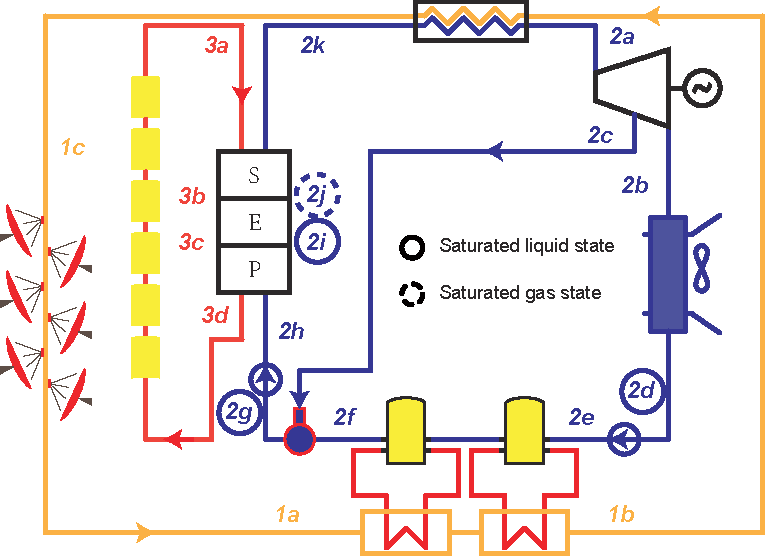
\includegraphics[width = 0.8\columnwidth]{fig/cascadeSystem}
	\caption{梯级系统结构示意图}
	\label{fig:System-1}
\end{figure}

梯级系统的水回路的$T$-$s$图如图\ref{fig:T-s_Water2}所示。在朗肯循环中,过程$2e$-$2f$的热量由斯特林机组提供,其传热过程曲线图如图\ref{fig:HeatTransfer_Water-SEs}所示。

\noindent \begin{figure}[htbp]
\centering
	\begin{subfigure}[b]{0.45\columnwidth}
	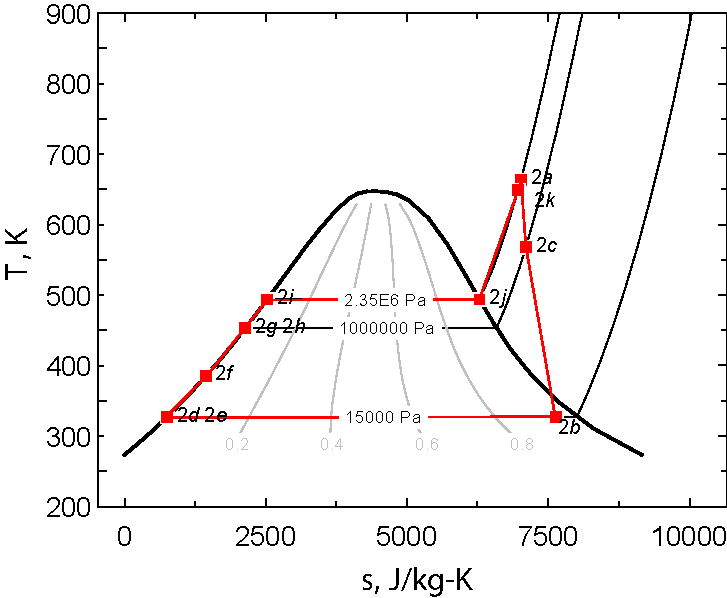
\includegraphics[width = \columnwidth]{fig/T-s_Water2}
	\caption{水循环的$T$-$s$图}\label{fig:T-s_Water2}
	\end{subfigure}
	~
\begin{subfigure}[b]{0.45\columnwidth}
	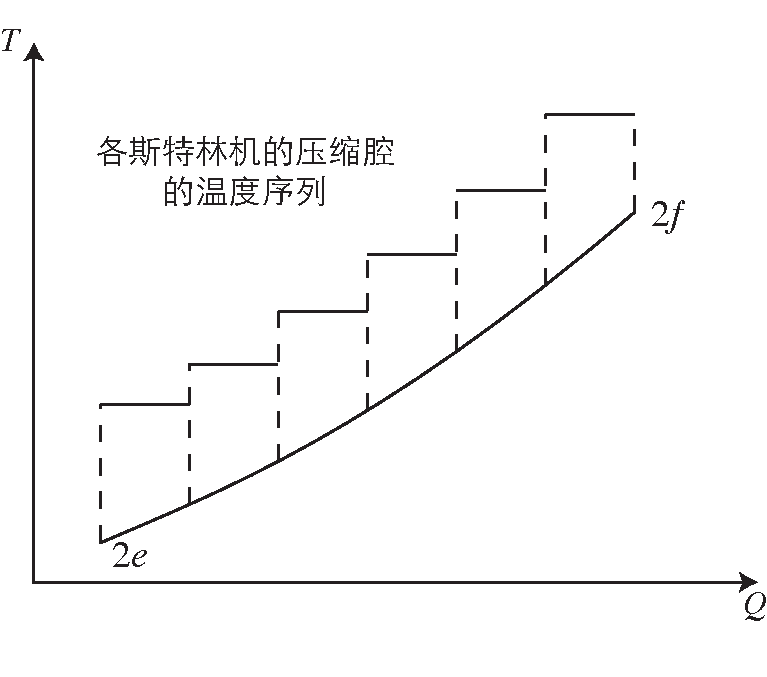
\includegraphics[width = \columnwidth]{fig/HeatTransfer_Water-SEs}
	\caption{$2e$-$2f$的传热过程曲线图}
	\label{fig:HeatTransfer_Water-SEs}
	\end{subfigure}
	
	\caption{水循环的过程曲线图和过程$2e$-$2f$的传热曲线图}\label{fig:Diagrams$2e$-$2f$}
\end{figure}

需要指出的是,第\ref{cha:osgs}章提出并分析了分段加热系统。分段加热系统比传统的蒸汽发生系统具有更好的热效率和㶲效率。然而,本章的梯级系统并没有使用该分段加热系统方案。这是因为,首先,为了更加清晰地表明本文所提出的梯级系统因梯级集热和梯级利用带来的收益,本章的梯级系统不使用分段加热系统。其次,同使用传统的蒸汽发生系统的太阳能光热发电系统相比,使用分段加热系统的太阳能光热发电系统只是改变了太阳能场部分。因此可以方便地将分段加热系统引入梯级系统而不影响其它部分的计算。最后,第\ref{cha:osgs}章提出的分段加热系统有很大的改进空间,值得以后进行更深入地研究。

\section{系统对比方案}

梯级系统评估的一个重要方面是与现有太阳能光热发电技术进行对比分析。对比分析主要有以下几种对比方案:

\begin{enumerate}[label=(\arabic*)]
	\item \emph{同槽式系统进行对比。} 

	\setlength\parindent{2em}当选择与槽式系统进行对比时,梯级系统获取的效率提升难以辨别出是由于采用梯级系统带来的提升还是只是由于采用了碟式集热器和斯特林机组带来的提升。
	\item \emph{同碟式系统进行对比。}
	
	当选择与碟式系统进行对比时,梯级效率获得的成本的降低难以区分是由于采用梯级系统带来的降低还是只是由于采用了槽式集热器和朗肯循环带来的降低。
	\item \emph{与多种系统同时对比。}
	
	一种自然的想法是,尽可能选用和梯级系统中相同的部件来组成对比系统。这意味,需要同时选择槽式-朗肯循环系统和碟式-斯特林机系统作为对比的系统。这两个系统独立存在,不存在梯级利用的关系,称为独立系统。
	
\end{enumerate}

\begin{figure}[htbp]
\centering
	\begin{subfigure}[b]{0.64\columnwidth}
	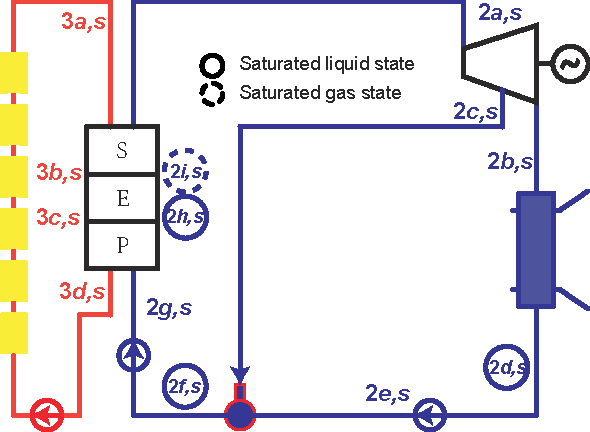
\includegraphics[width = \columnwidth]{fig/Trough-s}
	\caption{槽式-朗肯循环系统}\label{fig:TroughRankine}
	\end{subfigure}
	~
\begin{subfigure}[b]{0.26\columnwidth}
	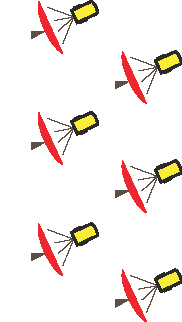
\includegraphics[width = \columnwidth]{fig/Dish-s}
	\caption{碟式-斯特林机系统}\label{fig:DishStirling}
	\end{subfigure}
	
	\caption{独立系统的结构示意图}\label{fig:Stand-alone-systems}
\end{figure}

	由于独立系统和梯级系统的不同,独立系统中的槽式集热器集热面积和汽轮机输出功不可能同时和梯级系统中的相同。同样,独立系统中的碟式集热器集热面积和斯特林机输出功不可能同时和梯级系统中的相同。
	
	如果以相同的汽轮机输出功和相同的斯特林机输出功作为选择独立系统的条件,独立系统将具有和梯级系统不同的槽式集热面积以及不同的碟式集热面积。然而,这将非常不利于未来对梯级系统进行经济性对比分析,因为槽式集热器单位面积的成本和碟式集热器单位面积的成本相差很大。
	
	一个更好的选择方案则是,以相同的槽式集热器和相同的碟式集热器作为选择独立系统的条件,这样可以利用发电设备的变工况运行来实现不更换设备而满足发电要求。同时,由于输出都是电能,可以很方便地进行效率对比分析和经济对比分析。

本文选用第三种对比方案,同时,以相同的槽式集热器和相同的碟式集热器作为选择独立系统的条件,即所选择的独立系统具有和梯级系统相同的槽式集热器和碟式集热器。
独立系统的结构示意图如图\ref{fig:Stand-alone-systems}所示。为了完成梯级系统的对比分析,利用系统建模方法,对两个独立系统分别进行建模工作。

\section{系统性能计算模型}
\subsection{梯级系统性能指标}

梯级系统同时使用不同类型的集热器和不同种类的热力循环,它们相互耦合在一起。无法评价某一种型式的集热器收集的能量所产生的电能及其光电转换效率。一个更加通用的选择是定义系统的整体效率。梯级系统的整体光电转换效率定义为总的输出功除以总的输入太阳能。
\begin{equation}
	\eta_{cs}=\dfrac{P_{cs}}{I_rA_{cs}} = \dfrac{P_{rk}+ P_{sea}}{I_rA_{tc} + I_rA_{dc}}
\end{equation}

其中,$P_{rk}$是朗肯循环的输出功率,$P_{sea}$是所有斯特林机的输出功率之和。
\begin{equation}
	P_{rk} = P_{tb} - P_{pu} / \eta_{ge}
\end{equation}

汽轮机的功率
\begin{equation}
  P_{tb}=\left(1-y\right)\dot{m}_{2}\left(h_{2a}-h_{2b}\right)+y\dot{m}_{2}\left(h_{2a}-h_{2c}\right)
\end{equation}

泵消耗的功率
\begin{equation}
	P_{pu}=\left(1-y\right)\dot{m}_{2}\left(h_{2e}-h_{2d}\right)+\dot{m}_{2}\left(h_{2h}-h_{2g}\right)
\end{equation}

依据能量守恒,斯特林机组的输出总功率等于单位时间内热流体的焓降减去热流体的焓升。
\begin{equation}
	P_{sea}=\dot{m}_1(h_{1,i,1} - h_{1,o,n_1}) - \dot{m}_2(h_{2,o,n_1} - h_{2,i,1})
\end{equation}

正如前文提到的,$\dfrac{P_{rk}}{I_rA_{tc}}$并不能表示槽式集热器的发电效率,$\dfrac{P_{sea}}{I_rA_{dc}}$也不能表示碟式集热器的发电效率。

\subsection{独立系统性能指标}

\subsubsection{独立槽式-朗肯循环系统}

在独立槽式-朗肯循环系统中,槽式集热器选取与梯级系统中相同的集热器。汽轮机、发电机、除氧器等部件用相同的部件以变工况的形式运行。
汽轮机的设计参数和相对内效率与梯级系统中的汽轮机一样。除氧器的工作压力与梯级系统中的一样。于是,图\ref{fig:Stand-alone-systems}中汽轮机的状态点$2b,s$和$2c,s$的参数可以由下式求出
\begin{equation}
	\eta_{i,tb}= (h_{2a,s}-h_{2b,s})/(h_{2a,s}-h_{i,2b,s}) = (h_{2a,s}-h_{2c,s})/(h_{2a,s}-h_{i,2c,s})
\end{equation}

汽轮机的输出功率
\begin{equation}
	P_{tb,s}=\left(1-y_{s}\right)\dot{m}_{2,s}\left(h_{2a,s}-h_{2b,s}\right)+y_{s}\dot{m}_{2,s}\left(h_{2a,s}-h_{2c,s}\right)
\end{equation}

发电机的输出功率
\begin{equation}
	P_{ge,s}=P_{tb,s}\eta_{ge}
\end{equation}

泵消耗的总功率
\begin{equation}
	P_{pu,s}=\left(1-y_{s}\right)\dot{m}_{2,s}\left(h_{2e,s}-h_{2d,s}\right)+\dot{m}_{2,s}\left(h_{2g,s}-h_{2f,s}\right)
\end{equation}

水循环的吸热量
\begin{equation}
	Q_{2,s}=\dot{m}_{2,s}\left(h_{2a,s}-h_{2g,s}\right)
\end{equation}

发电机的效率和梯级系统中发电机的效率相同,所以朗肯循环的效率可以表示为
\begin{equation}
	\eta_{rk,s}=(P_{tb,s}-P_{pu,s}/\eta_{ge})/Q_{2,s}
\end{equation}

\subsubsection{独立碟式-斯特林机系统}

在独立碟式-斯特林机系统中,碟式集热器选取与梯级系统中相同的集热器。
为了和现有技术进行对比,将具有和碟式集热器相同数目的斯特林机放置于各碟式集热器的焦点处。斯特林机利用水来冷却。$T_{H,s}$选择为碟式集热器出口的空气温度,即1073$\,\mathrm{K}$。$T_{L,s}$依据Fraser的论文\cite{Fraser2008}中的默认膨胀腔的温度数据选定为310$\,\mathrm{K}$。$k$和$\gamma$选择和梯级系统中的斯特林机相同。

由于冷热流体的改变(冷流体改用了冷却水,选用固定膨胀腔温度的方式进行计算;取消了热流体,而采用太阳辐射直接照射的方式让斯特林机直接从太阳辐射中获取能量),本文建立的斯特林机模型不能应用于该独立碟式-斯特林机系统中的斯特林机。采用经典的斯特林机模型公式来计算斯特林机的效率\cite{Stine1998}:
\begin{equation}
	\eta_{sea,s}=\dfrac{T_{H,s}-T_{L,s}}{T_{H,s}+\dfrac{1-e_{s}}{k-1}\cdot\dfrac{T_{H,s}-T_{L,s}}{\ln\gamma}}
\end{equation}
其中,$T_{R,s}=\dfrac{T_{H,s}-T_{L,s}}{\ln(T_{H,s}/T_{L,s})}$,$e_{s}=\dfrac{T_{R,s}-T_{L,s}}{T_{H,s}-T_{L,s}}$。

斯特林机组的总输出功率为
\begin{equation}
	P_{sea,s}=n_{dc}A_{dc}I_r\eta_{dc}\eta_{sea,s}
\end{equation}

\section{系统参数设置}

为了研究梯级系统的性能及其影响因素,需要对系统进行建模仿真分析。第\ref{cha:Modeling}章详细介绍了系统的建模方法。利用太阳能光热系统设计软件完成系统建模后,另一项重要的任务就是确定系统的参数。

系统中的参数主要由以下部分确定:

\begin{enumerate}[label=(\arabic*)]

\item 环境

\setlength\parindent{2em}典型的环境参数值设定为:
$I_r = 700\,\mathrm{W/m^2}$,$T_{amb} = 293\,\mathrm{K}$,$p_{amb} = 1\times10^5\,\mathrm{Pa}$,$v_{amb} = 1\,\mathrm{m/s}$。

\item 汽轮机

汽轮机以青岛捷能汽轮机集团股份有限公司的N-6 2.35系列产品为设计原型。其额定参数为:$P = 6\,\mathrm{MW}$,$p_s = 2.35\,\mathrm{MPa}$,$T_s = 390\mathrm{^\circ C}$,$\dot{m} = 32.09\,\mathrm{t/h}$,$p_c = 0.015\,\mathrm{MPa}$,$s_{tb} = 3000\,\mathrm{rpm}$。
	
	已知主汽参数,其比焓和比熵可以通过物性参数插件CoolProp获得:$h_s = 3.2203\times10^6\,\mathrm{J/kg}$,$s_s = 7.0149\times10^3\,\mathrm{J/(kg\cdot K)}$。
	
	汽轮机的排汽焓:$h_{c} = h_{s} - \dfrac{P}{\dot{m}} = 2.5472\times10^6\,\mathrm{J/kg}$。
	
	已知排汽压力以及$s_{i,c} = s_s$,汽轮机的理想排汽焓值可以由CoolProp获得:$h_{i,c} = 2.2737\times10^6\,\mathrm{J/kg}$。
	
	所以,汽轮机的相对内效率
	$\eta_{i,tb} = \dfrac{h_s - h_c}{h_{s} - h_{i,c}} = 0.71$。
	
	考虑到适用于本文提出的梯级系统,汽轮机的参数选择值见表\ref{tab:CascadeSystemParameters}。
		 
\item 槽式集热器

由于LUZ公司的LS-3型号的集热器的实验数据比较丰富,本文选用它作为槽式集热器。它的主要参数见表\ref{tab:TroughParameters}~\cite{Fernandez2010}。

\begin{table}[htbp]
\setlength{\abovecaptionskip}{0pt}
	\caption{LS-3型槽式集热器的主要参数}
	\centering
	\begin{tabular}{cccccc}
		\toprule
		参数		&	值	&	参数		&	值	&	参数		&	值\\
		\midrule
		$A_{pc}$		&	$570.2\,\mathrm{m^2}$	&	$w_{dc}$	&	$5.76\,\mathrm{m}$	&	$L_{dc}$	&	$99\,\mathrm{m}$\\
		$f$	&	$1.71\,\mathrm{m}$	&	$d_i$		&	$0.066\,\mathrm{m}$	&	$d_o$	&	$0.07\,\mathrm{m}$\\
		$d_{abs,i}$	&	$0.113\,\mathrm{m}$	&	$d_{abs,o}$	&	$0.115\,\mathrm{m}$	&	Rim angle	&	$80^\circ$\\
		$\epsilon$		&	$0.15$	&	$\eta_{peak}$	&	$0.77$	&	$\rho$	&	$0.94$\\
		$\tau$	&	$0.95$	&	
$\alpha$	&	$0.96$	&	$Fe$	&	$0.97$\\
		\bottomrule
	\end{tabular}
	\label{tab:TroughParameters}
\end{table}

\item 碟式集热器

碟式集热器的反射镜选用SES公司的产品,而碟式接收器采用自行设计的方案。碟式集热器的反射镜参数和接收器参数见表\ref{tab:dc}。

\item 斯特林机

梯级系统所用的斯特林机和第\ref{sec:StirlingEngineModel}节中分析的斯特林机相同,即GPU-3型斯特林机,其参数见表\ref{tab:GPU3parameters}。

\item 预热器

水在预热器中由过冷水被加热成饱和液态水,水在预热器的出口干度为0 ($x = 0$)。

此外,考虑到夹点温度,预热器的入口油温要比出口水温高出$\Delta T_{min}$,即$T_{3c} - T_{2i} = \Delta T_{min}$,$\Delta T_{min}$设定为$15\,\mathrm{K}$。

\item 蒸发器

水在蒸发器中由饱和液态水被加热成饱和蒸汽,水在蒸发器的出口干度为1 ($x = 1$)。

\item 过热器

过热器的入口油温受限于导热油的属性。在梯级系统中,导热油选用Therminol VP-1型合成油,它的物性参数可以通过CoolProp得到。过热器的入口油温设定为$T_{3a} = 623\,\mathrm{K}$。

\item 除氧器

除氧器具有两股入口流体和一股出口流体,它们都具有相同的压力。设定除氧器的压力$p_e = 1\times10^6\,\mathrm{Pa}$。除氧器的出口流体为饱和液态水,其干度为0 ($x = 0$)。

\item 空气-水换热器

空气-水换热器的入口空气温度设定为 $T_{1b} = 673\,\mathrm{K}$。
\end{enumerate}

\smallskip{}
梯级系统的主要设计参数归纳见表\ref{tab:CascadeSystemParameters}。

\begin{table}[htbp]
\setlength{\abovecaptionskip}{0pt}
	\caption{梯级系统的基本设计参数}
	\centering
	\begin{tabular}{cccccc}
		\toprule
		参数		&	值	&	参数		&	值	&	参数		&	值\\
		\midrule
		$I_r$		&	$700\,\mathrm{W/m^2}$	&	$T_{dc,o}$	&	$1073\,\mathrm{K}$	&	$n_{se}$	&	100\\
		$T_{amb}$	&	$293\,\mathrm{K}$	&	$p_{dc}$		&	$5\times10^5\,\mathrm{Pa}$	&	$T_s$	&	$613\,\mathrm{K}$\\
		$p_{amb}$	&	$1\times10^5\,\mathrm{Pa}$	&	$\Delta{}T_{3,2,min}$	&	$15\,\mathrm{K}$	&	$p_s$	&	$2.35\times10^6\,\mathrm{Pa}$\\
		$v_{amb}$	&	$1\,\mathrm{m/s}$	&	$T_{tc,o}$	&	$623\,\mathrm{K}$	&	$p_c$	&	$1.5\times10^4\,\mathrm{Pa}$\\
		$P_{ge}$	&	$6\times10^6\,\mathrm{W}$	&	
$p_{tc}$	&	$2\times10^6\,\mathrm{Pa}$	&	$T_{s,d}$	&	$663\,\mathrm{K}$\\
		$T_{dc,i}$		&	$623\,\mathrm{K}$	&	$T_{1b}$	&	$673\,\mathrm{K}$	&	$p_{de}$ 	& 	$1\times10^6\,\mathrm{Pa}$\\
	\bottomrule
	\end{tabular}
	\label{tab:CascadeSystemParameters}
\end{table}

\section{同独立系统的对比分析}

在设计参数条件下,经过系统建模和仿真,得到梯级系统和其对应的独立系统的结果如表\ref{tab:importantResults}所示。其中,梯级系统的斯特林机组采用串联逆流的排列方式(第3种基本排列方式)。可以发现,在设计参数条件下,梯级系统可以获得比其对应的独立系统更高的光热发电效率。尽管梯级系统斯特林机组的效率较低,但朗肯循环的效率更高。梯级系统可以获得额外$3.83\times10^4\,\mathrm{W}$的功率输出。

\begin{table}[htbp]
\setlength{\abovecaptionskip}{0pt}
	\caption{设计参数下,梯级系统和其对应的独立系统的模拟分析结果}
	\centering
	\begin{tabular}{p{1cm}<{\centering} p{1.75cm}<{\centering} p{1cm}<{\centering} p{1.75cm}<{\centering} p{1cm}<{\centering} p{3cm}<{\centering}}
		\toprule
		参数		&	值	&	参数		&	值	&	参数		&	值\\
		\midrule
		$\eta_{cs}$		&	0.1974	&	$\eta_{sea,s}$	&	0.3786	&	$P_{ge,s}$	&	$5.826\times10^6\,\mathrm{W}$\\
		$\eta_{s}$	&	0.1962	&	$\eta_{rk}$	&	0.2660	&	$P_{sea}$		&	$3.552\times10^5\,\mathrm{W}$\\
		$\eta_{diff}$		&	0.0062	&	$\eta_{rk,s}$	&	0.2678	&	$P_{sea,s}$	&	$4.909\times10^5\,\mathrm{W}$\\
		$\eta_{sea}$	&	0.3407	&	$P_{ge}$		&	$6\times10^6\,\mathrm{W}$	&	$P_{diff}$		&	$3.830\times10^4\,\mathrm{W}$\\
		\bottomrule
	\end{tabular}
	\label{tab:importantResults}
\end{table}

接下来的各小节分析在不同因素的影响下,梯级系统与其对应的独立系统之间的效率差异$\eta_{diff}$的分析。
\subsection{法向直射强度$I_r$的影响}
\label{sec:I_r}

法向直射强度$I_r$对梯级系统和独立系统都有影响,因此对两种系统的效率差异($\eta_{diff}$)也会有影响。$I_r$对$\eta_{diff}$的影响曲线图如图\ref{fig:I_r-eta_diff}所示。从图中可以发现,对于较高的辐射强度($I_r > 550\,\mathrm{W/m^2}$),$\eta_{diff}>0$,梯级系统可以获得更高的光电转换效率。对于较低的辐射强度($I_r < 550\,$W/m$^2$),$\eta_{diff}$可能为负值。在这种条件下,梯级系统的光电转换效率要低于其对应的独立系统。这可以被解释为,由于梯级系统使用朗肯循环的给水来冷却斯特林机,随着给水温度的升高,这种冷却方式将会削弱斯特林机的冷却效果,导致斯特林机功率和效率的下降。对于较低的辐射强度,汽轮机功率的增加量要小于斯特林机组因此带来的功率损失。而随着辐射强度的增大,凝结水吸收的热量给汽轮机带来的功率提升逐渐高于斯特林机的功率损失。此外,在高辐射强度的条件下,不同型式的集热器具有更显著的集热性能差异,更能体现出梯级集热带来的益处。所以,太阳法向直射强度$I_r$较高的地区更适合采用梯级系统。这意味着太阳法向直射强度是梯级系统选址所需要考虑的一个重要因素。
\begin{figure}[htbp]
	\centering
	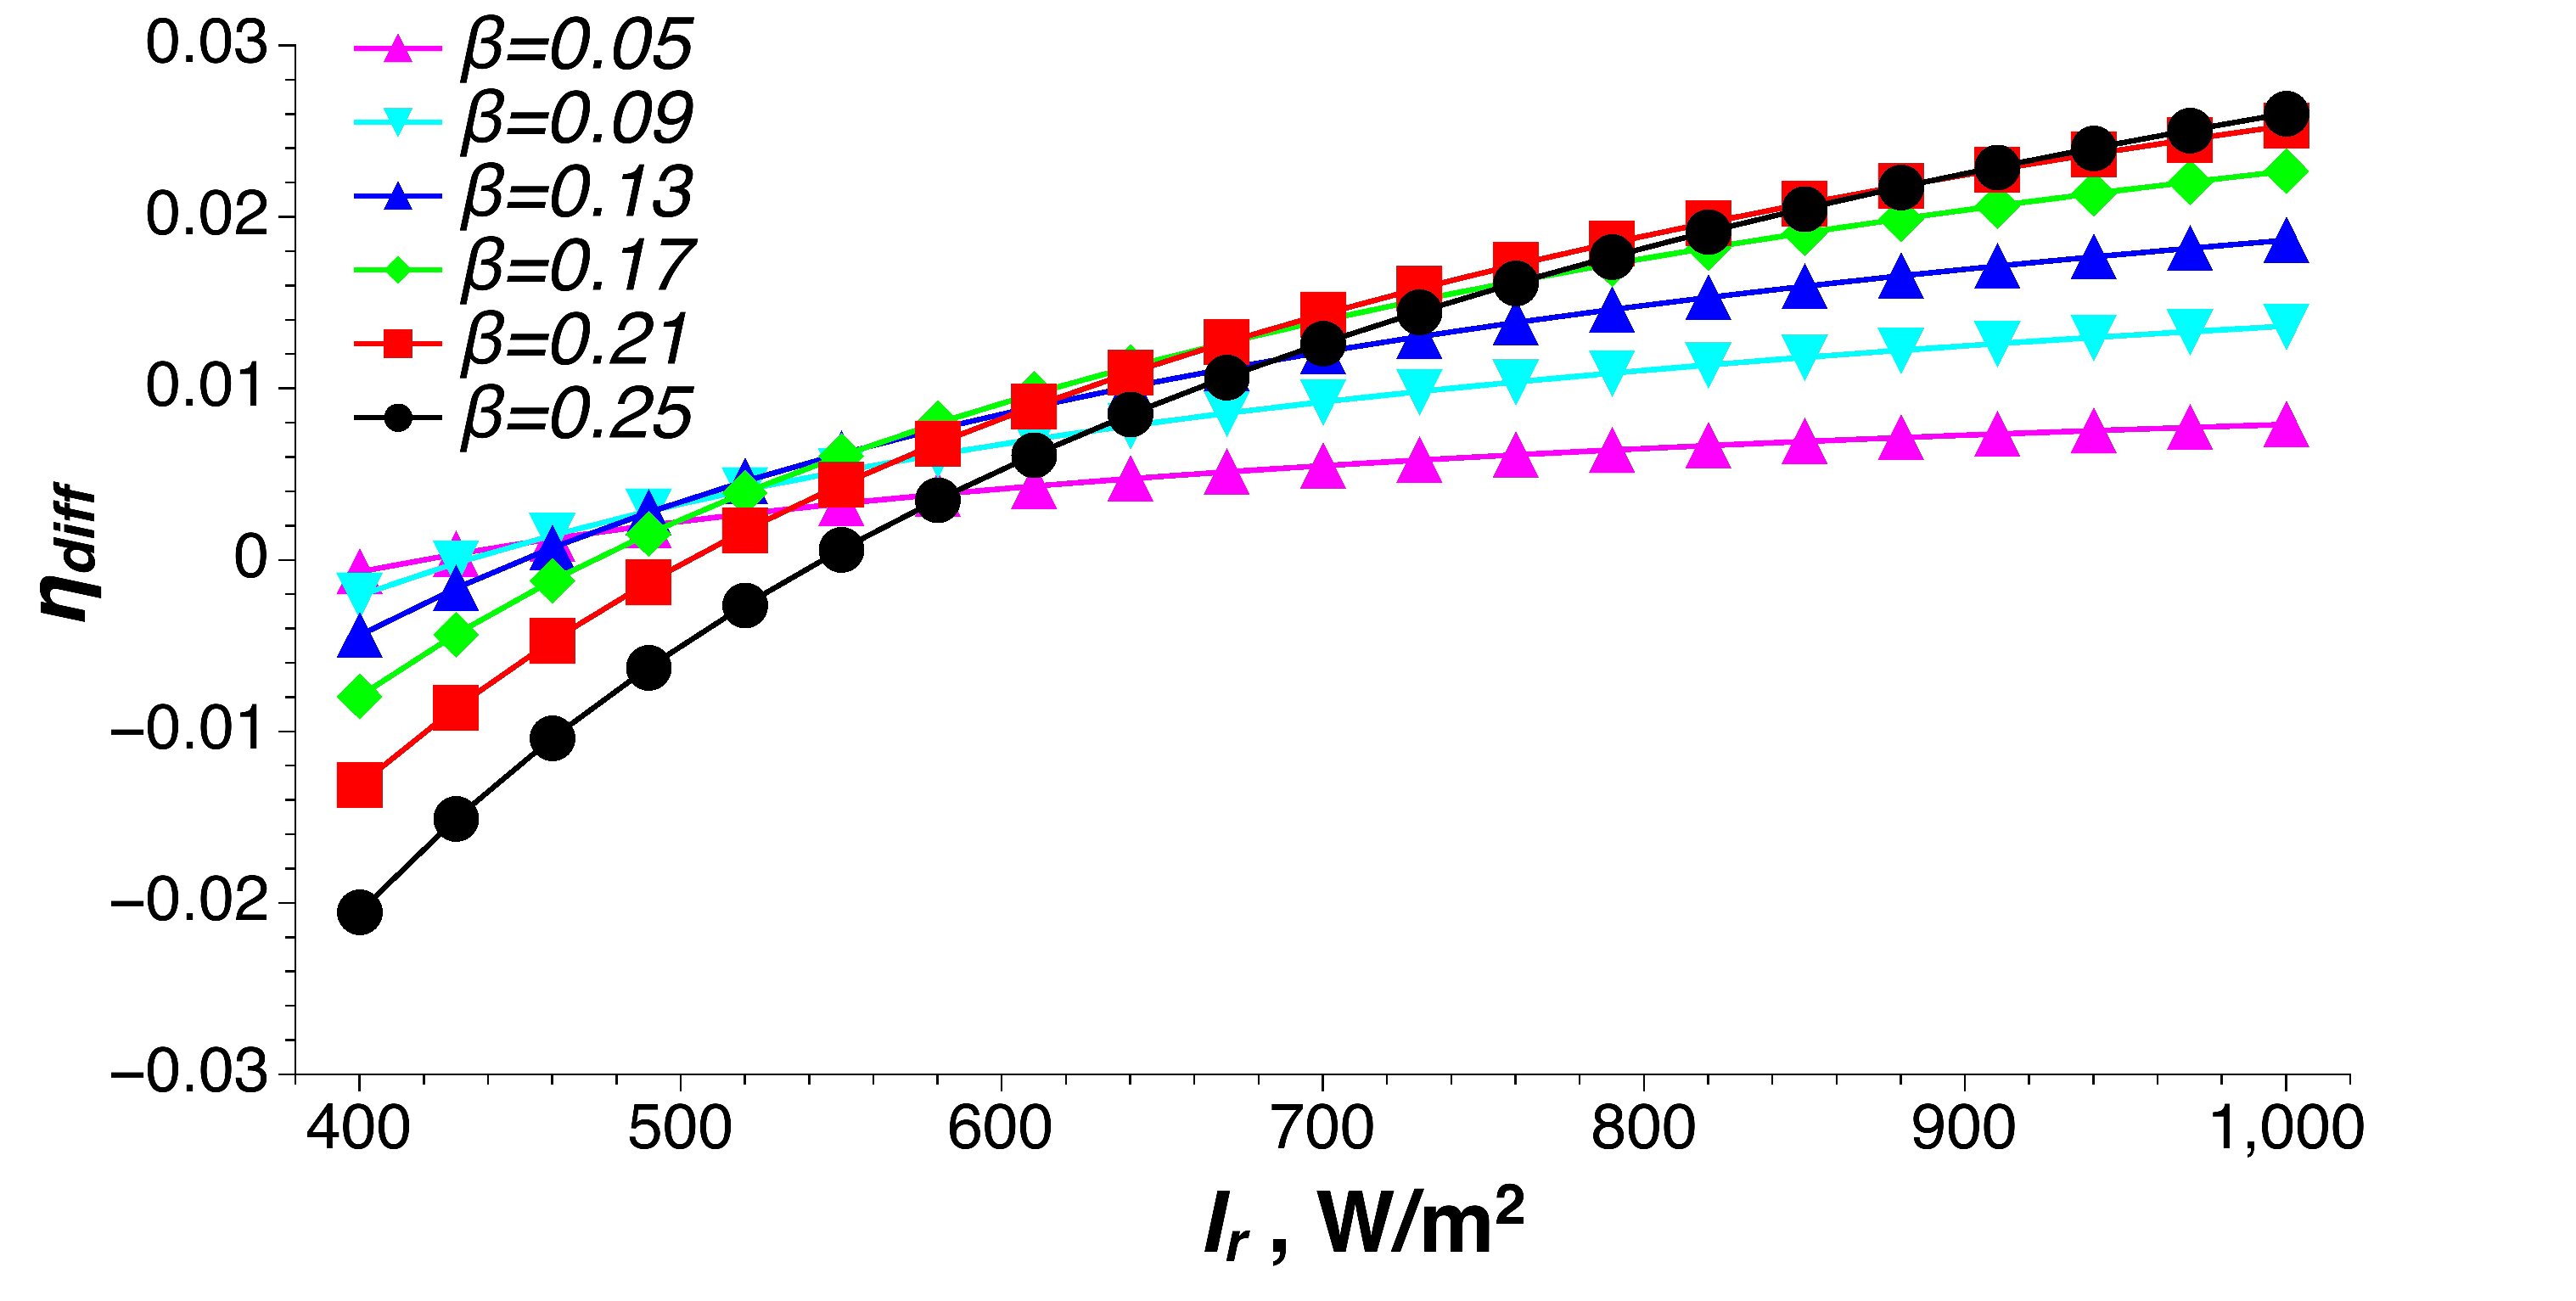
\includegraphics[width = 0.9\columnwidth, angle = 0]{fig/I_r-eta_diff}
	\caption{法向直射强度$I_r$对$\eta_{diff}$的影响曲线图}
	\label{fig:I_r-eta_diff}
\end{figure}

\subsection{斯特林机发电比例$\beta$的影响}

表\ref{tab:importantResults}中的结果表明,在设计参数条件下,梯级系统带来的效率提升非常低。其中的一个原因就是斯特林机发电功率占系统发电总功率的比例$\beta$太小。这样被朗肯循环给水吸收的斯特林机组释放的热量只占朗肯循环吸收总热量的一小部分,梯级利用的效果并不明显。所以,增加$\beta$可以增加梯级利用的效果,可能会获得更大的$\eta_{diff}$。不同太阳辐射强度条件下的$\beta$对$\eta_{diff}$的影响如图\ref{fig:beta-eta_diff}所示。可以发现,对于较高的太阳法向直射辐射,增加$\beta$可以获得更高的效率提升,但是,这个提升存在极限值。对于$I_r=900$W/m$^2$,当$\eta_{diff}=0.0228$时,获得最大效率提升值$\eta_{diff}=0.0228$。对于较低的太阳法向直射辐射,$\eta_{diff}$为负值,增加$\beta$将会进一步减小$\eta_{diff}$。这可以解释为,$\beta$的增大将会恶化斯特林机组的散热,使斯特林机组性能下降。

\begin{figure}[H]
\centering
	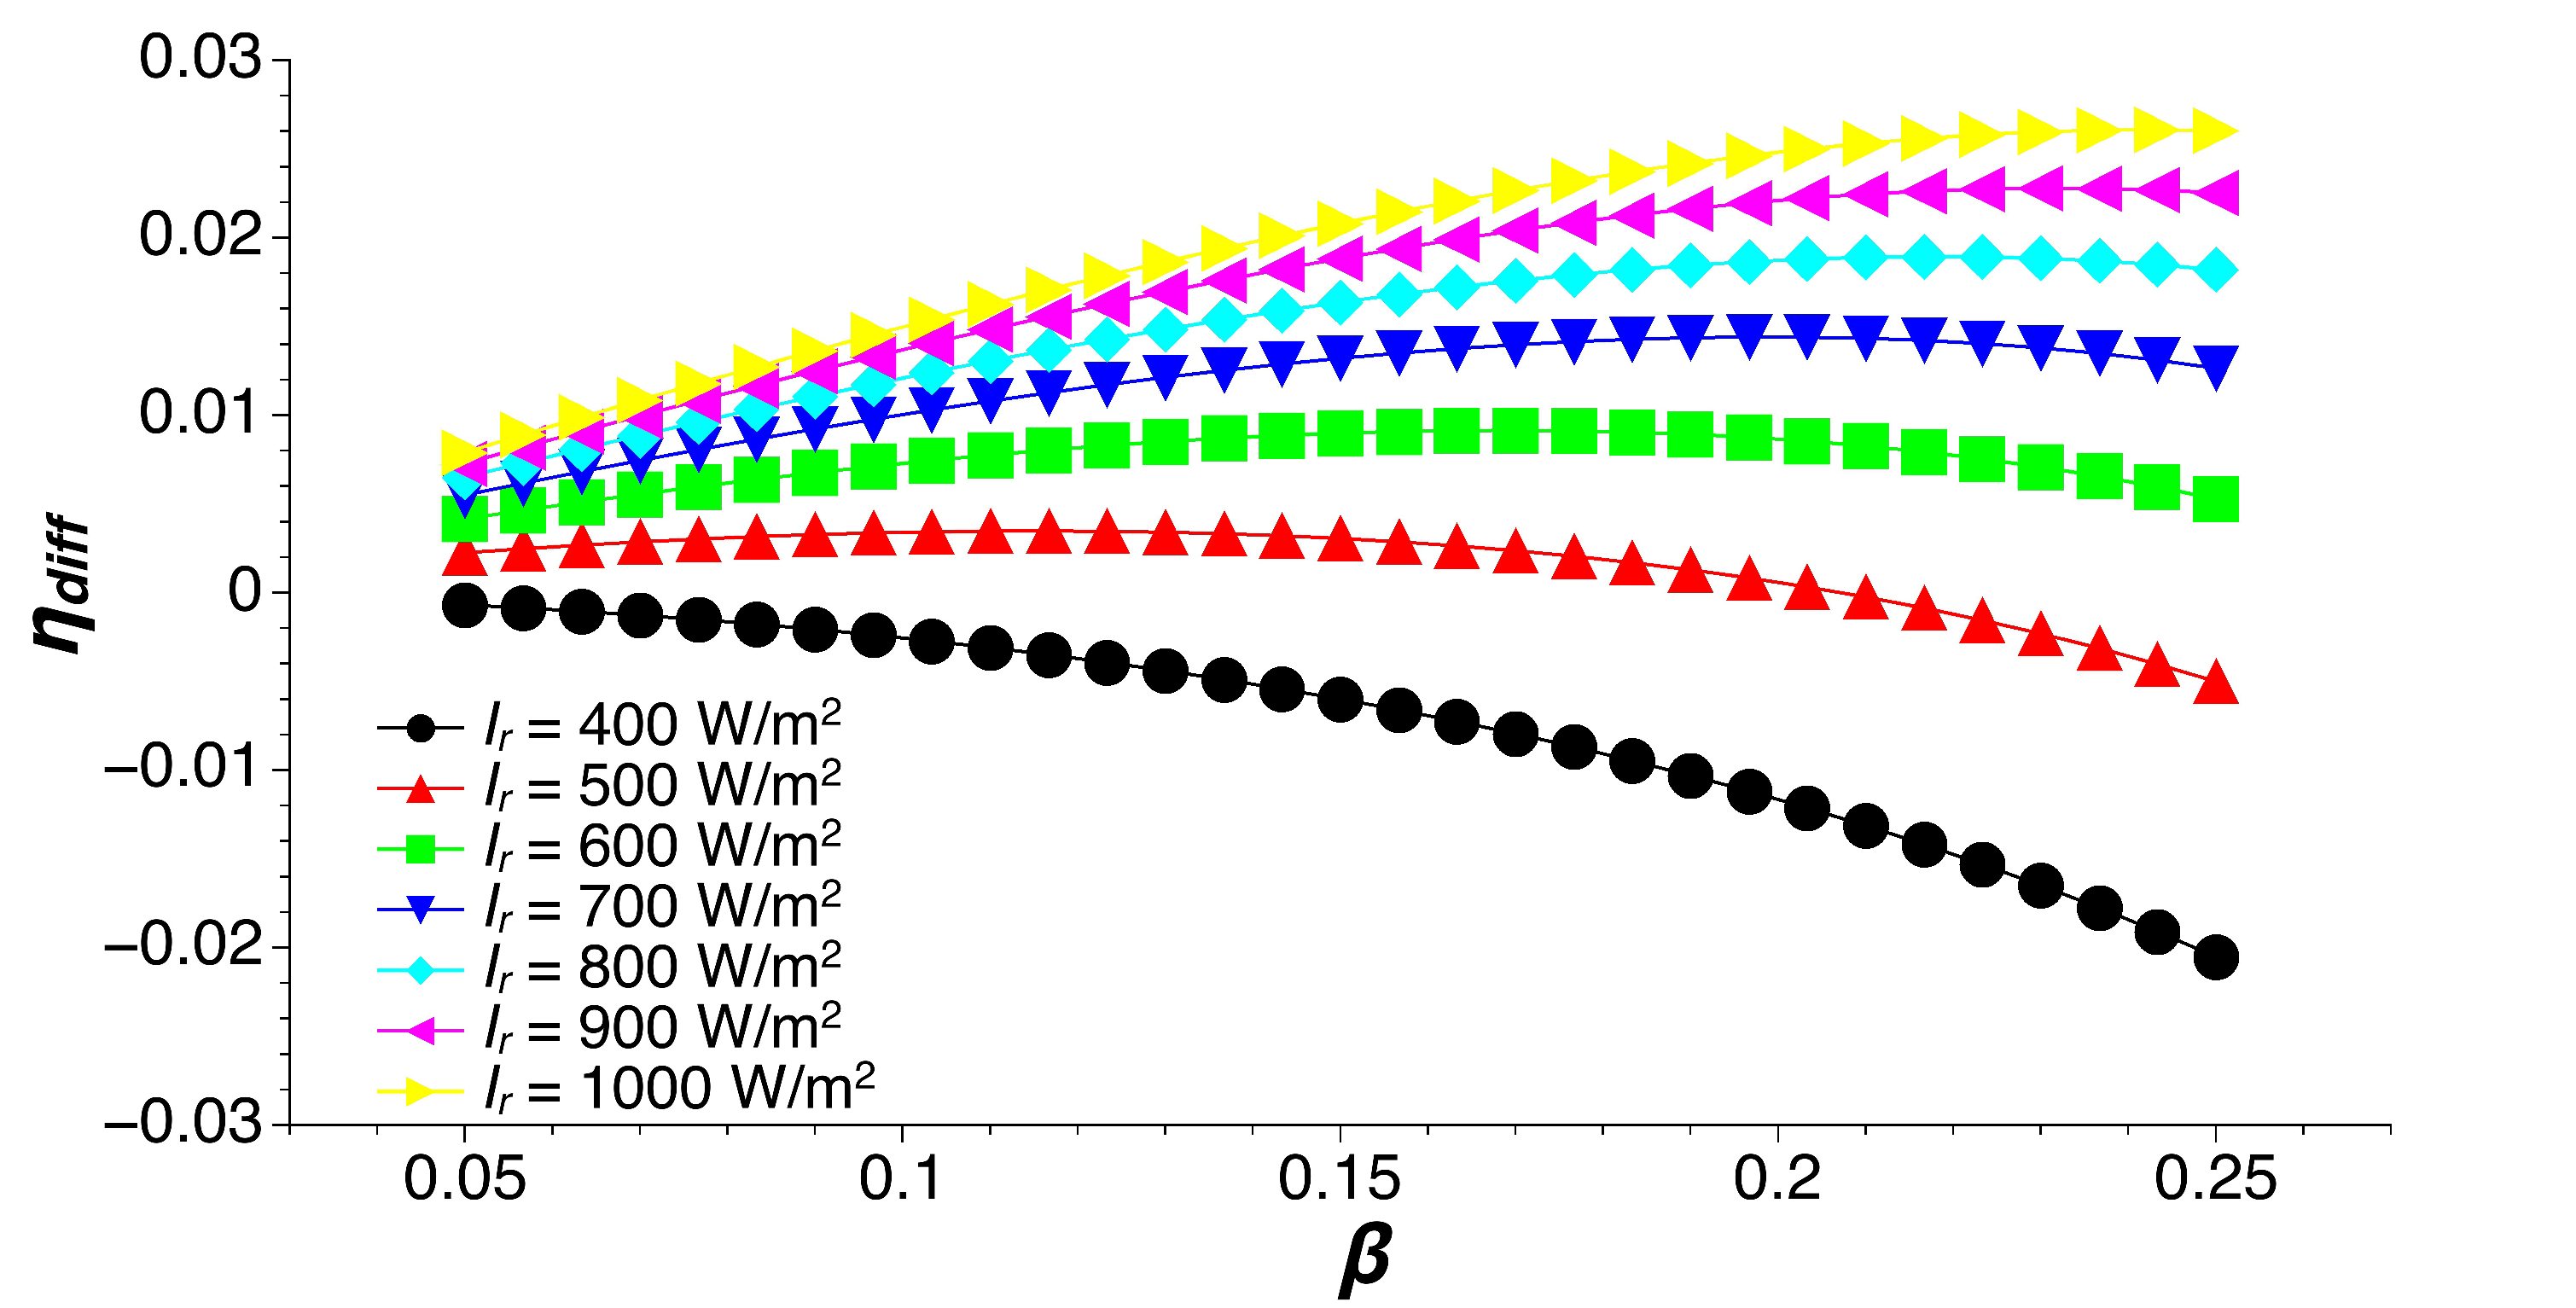
\includegraphics[width = 0.8\columnwidth, angle = 0]{fig/beta-eta_diff}
	\caption{斯特林机发电比例$\beta$对$\eta_{diff}$的影响曲线图}
	\label{fig:beta-eta_diff}
\end{figure}

\subsection{冷热流体流动方向的影响}

正如第\ref{cha:optSEA}章中提到的,斯特林机组的排列方式对系统的发电效率有影响。采用串联连接是最好的连接方式。本小节研究在串联连接的条件下,冷热流体流动方向(顺流逆流)对$\eta_{diff}$的影响。同逆流相比,顺流会导致前面的斯特林机的功率和效率更高,而后面的斯特林机的功率和效率更低。

\begin{table}[htbp]
\setlength{\abovecaptionskip}{0pt}
	\caption{斯特林机组采用不同流体流动方向时的模拟结果}
	\centering
	\begin{tabular}{ccccccccc}
		\toprule
		\multirow{3}{*}{$x$}	&	\multicolumn{4}{c}{顺流}	&\multicolumn{4}{c}{逆流}\tabularnewline
		\cline{2-5}	\cline{6-9}
		&$T_{1,i}$&$T_{2,i}$&$P_{sea}$&$\eta_{sea}$&$T_{1,i}$&$T_{2,i}$&$P_{sea}$&$\eta_{sea}$\tabularnewline
		&K&K&W&-&K&K&W&-\tabularnewline
		\midrule
		1	&	1073.15	&	327.17	&	5000	&	0.3648	&	1073.15	&	348.09	&	4867	&	0.3601\\
		2	&	1022.38	&	329.80	&	4630	&	0.3599	&	1023.25	&	345.48	&	4541	&	0.3562\\
		3	&	974.35	&	332.29	&	4280	&	0.3544	&	975.82	&	343.00	&	4230	&	0.3520\\
		4	&	928.90	&	334.65	&	3949	&	0.3485	&	930.75	&	340.65	&	3934	&	0.3474\\
		5	&	885.91	&	336.88	&	3635	&	0.3419	&	887.94	&	338.42	&	3654	&	0.3424\\
		6	&	845.26	&	339.00	&	3338	&	0.3347	&	847.28	&	336.29	&	3387	&	0.3370\\
		7	&	806.82	&	341.00	&	3057	&	0.3269	&	808.69	&	334.28	&	3134	&	0.3312\\
		8	&	770.49	&	342.91	&	2792	&	0.3184	&	772.06	&	332.37	&	2894	&	0.3248\\
		9	&	736.16	&	344.71	&	2541	&	0.3090	&	737.31	&	330.55	&	2666	&	0.3180\\
		10	&	703.75	&	346.43	&	2304	&	0.2989	&	704.37	&	328.82	&	2450	&	0.3106\\
		\bottomrule
	\end{tabular}
	\label{tab:SEAresults}
\end{table}

两种不同流体流动方向的模拟结果见表\ref{tab:SEAresults}。冷热流体在不同斯特林机处的温度以及不同斯特林机的效率的拟合曲线如图\ref{fig:Parallelflow}和图\ref{fig:Counterflow}所示。

\begin{figure}[ht!]
\centering
	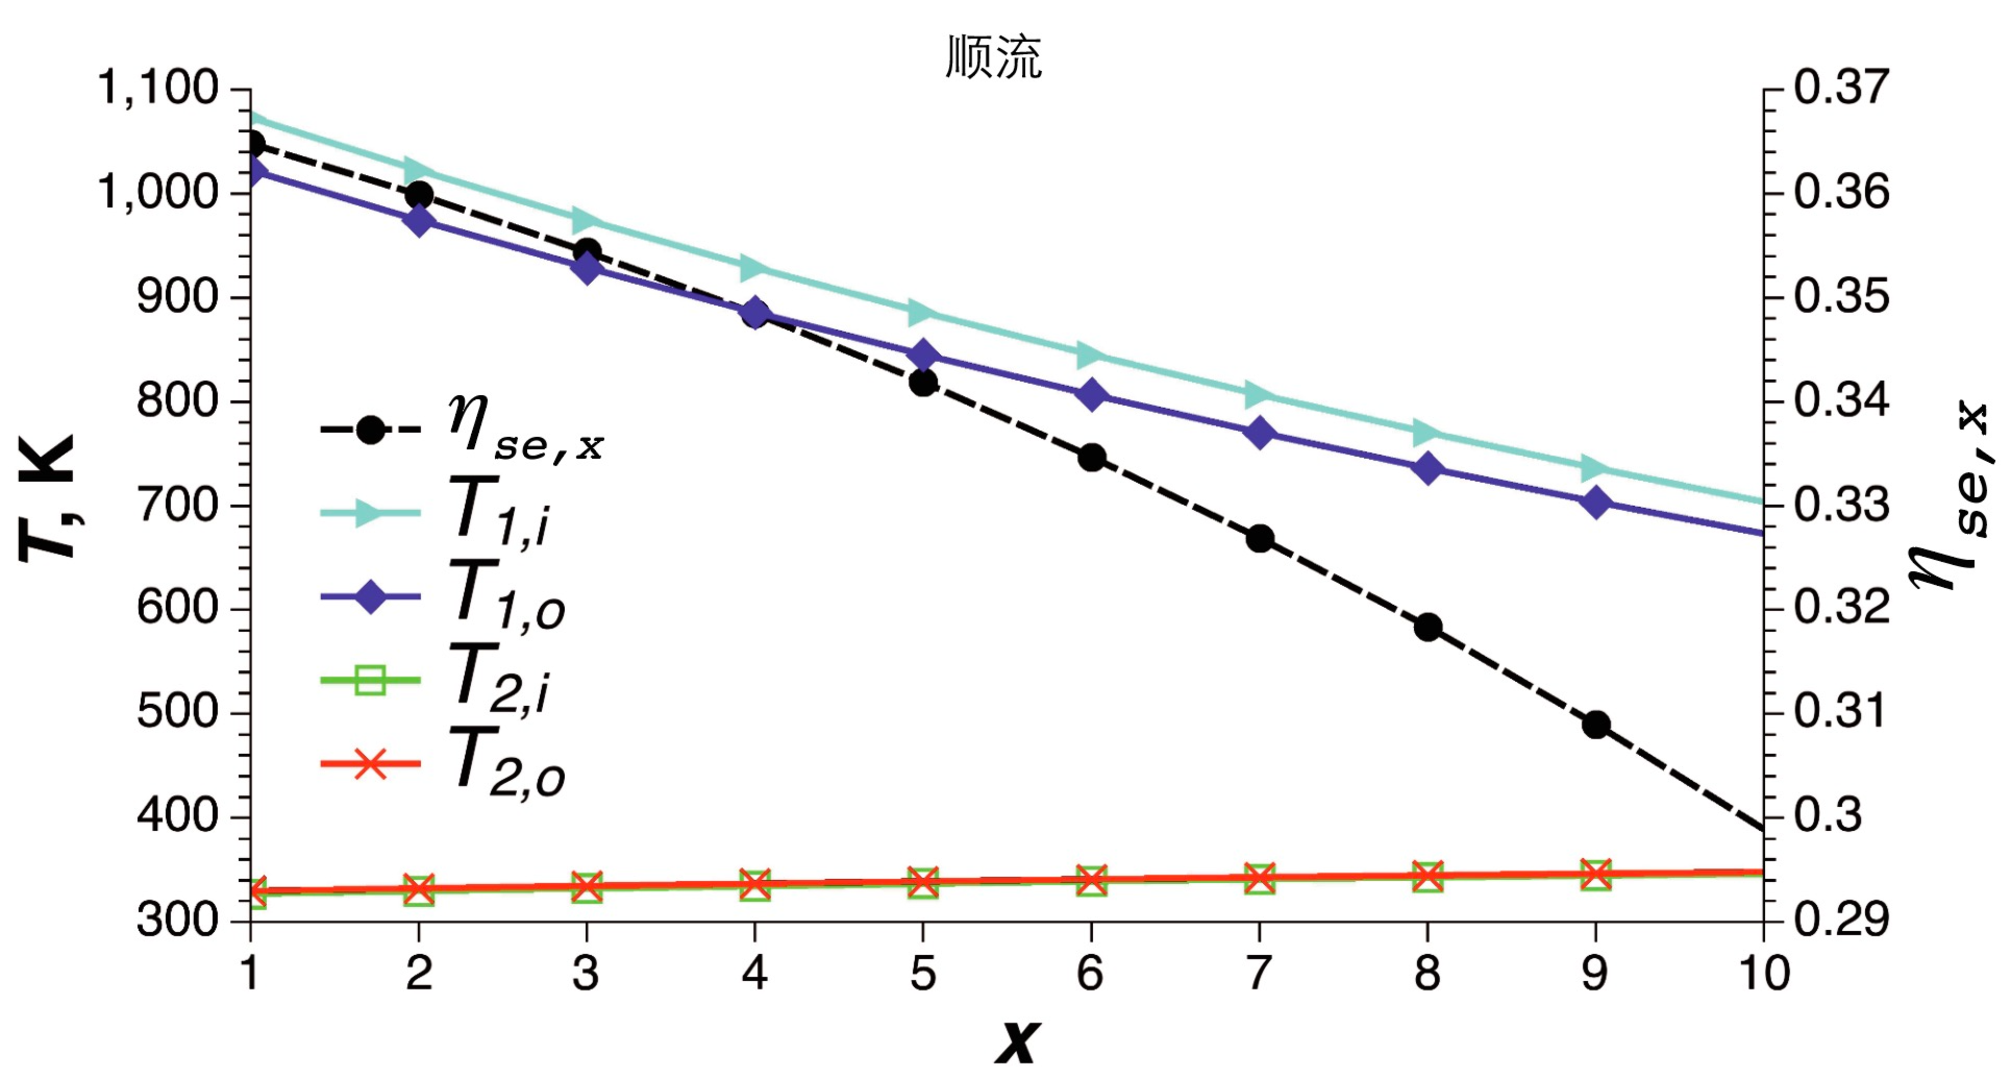
\includegraphics[width = 0.8\columnwidth]{fig/Parallelflow.pdf}
	\caption{顺流时,各斯特林机的效率及其进出口流体温度的拟合曲线图}
	\label{fig:Parallelflow}
\end{figure}

\begin{figure}[ht!]
\centering
	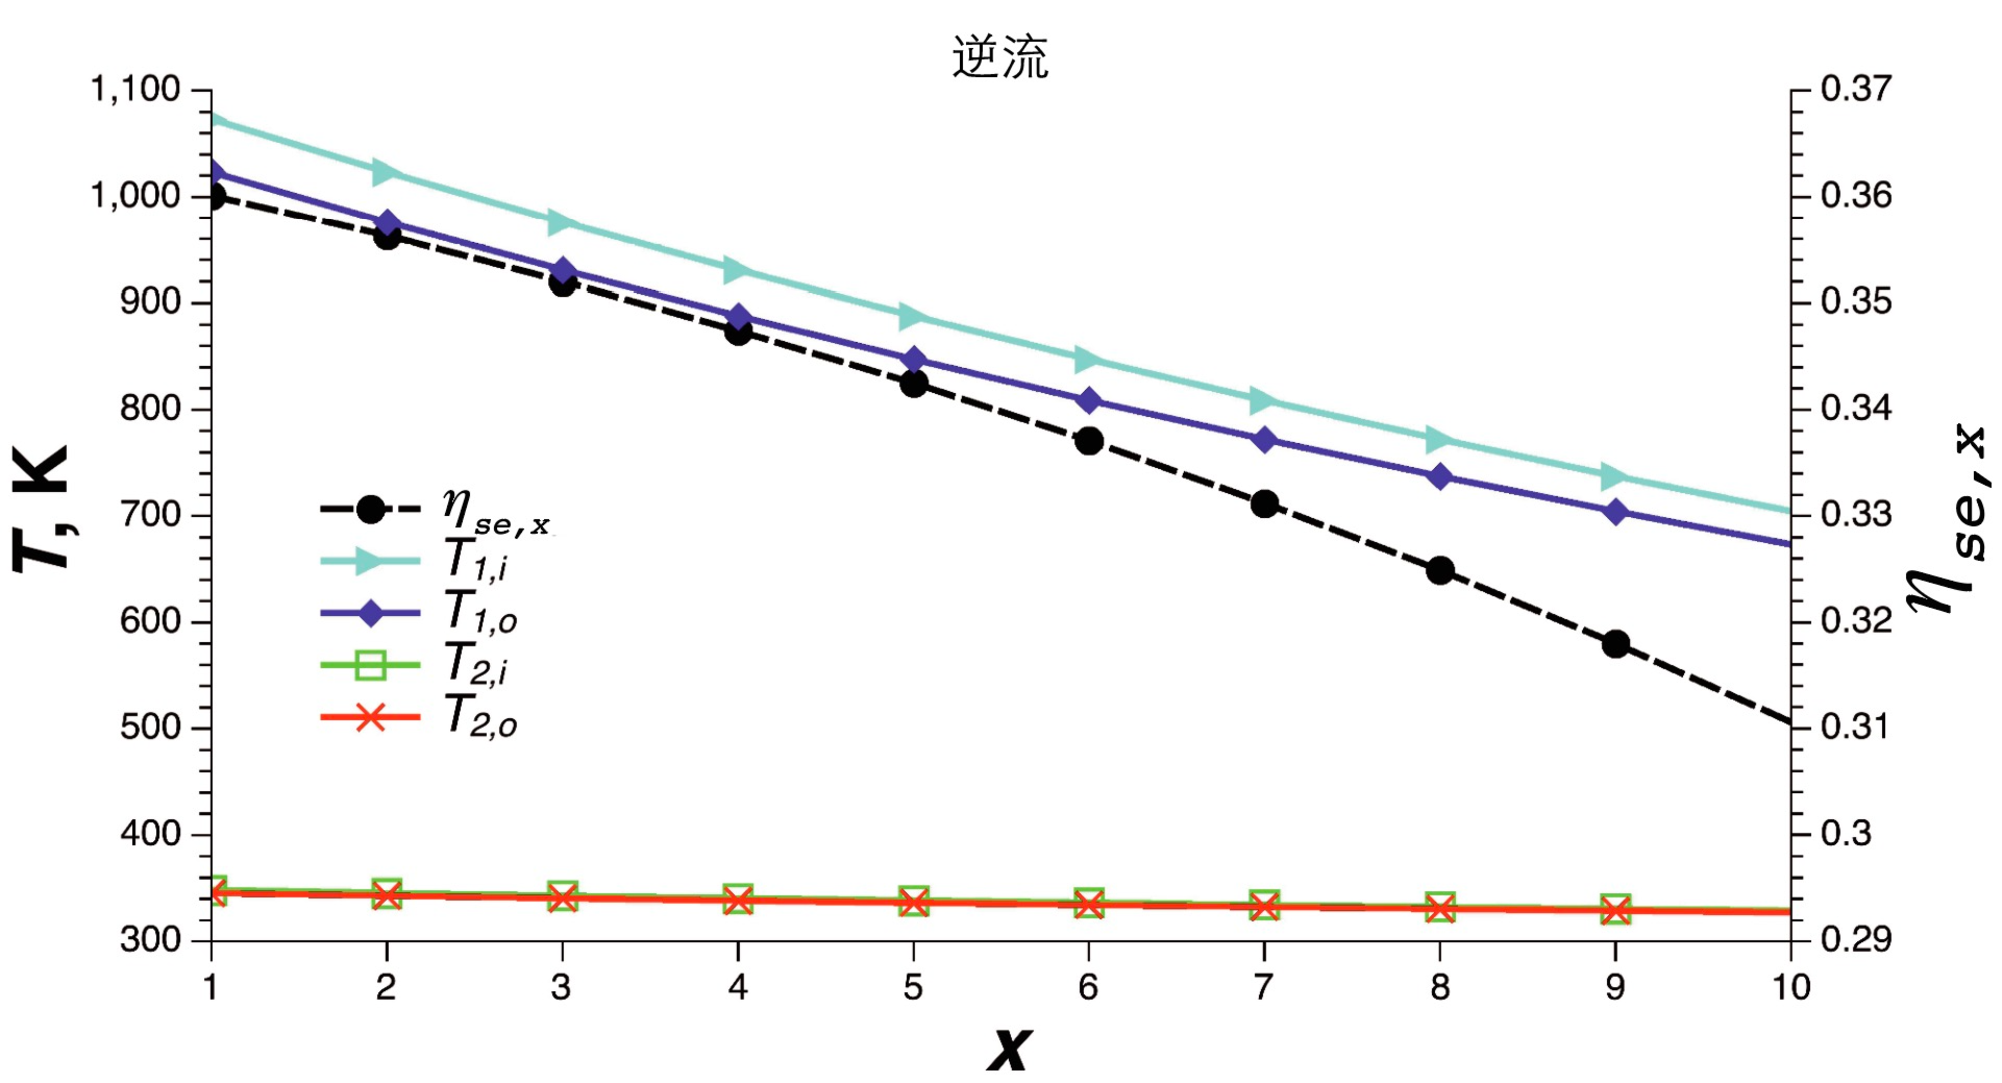
\includegraphics[width = 0.8\columnwidth]{fig/Counterflow.pdf}
	\caption{逆流时,各斯特林机的效率及其进出口流体温度的拟合曲线图}
	\label{fig:Counterflow}
\end{figure}

可以发现,相比于热流体温度变化量,冷流体的温度增量非常小,这是因为冷流体(水)具有大得多的热容量$\dot{m}c_p$。这也使得两种流动方向的斯特林机组的性能差异很小。

\begin{figure}[htbp]
\centering
	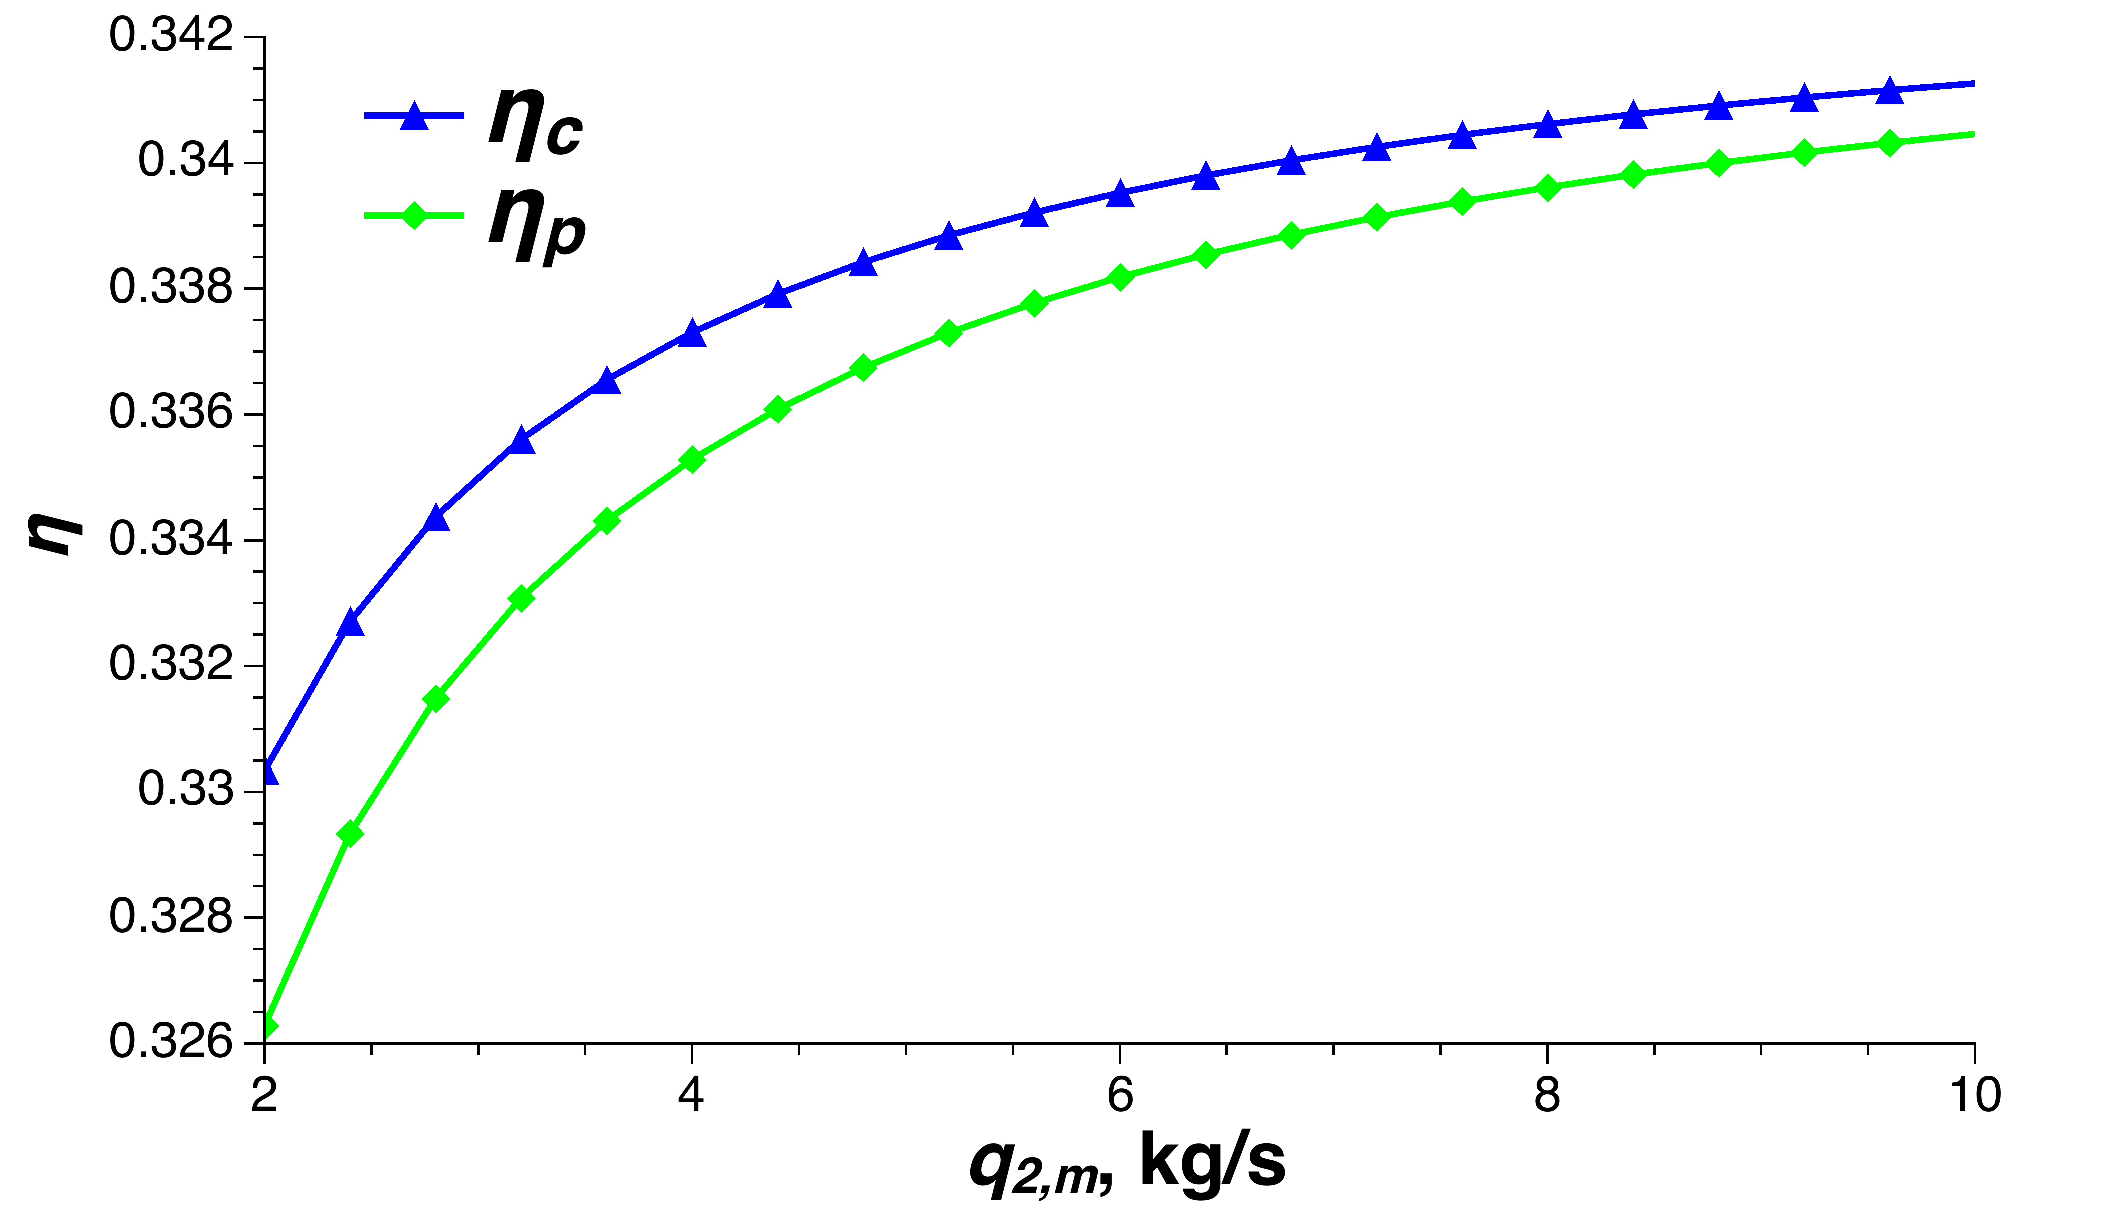
\includegraphics[width = 0.8\columnwidth, angle = 0]{fig/SEAflowtypes}
	\caption{斯特林机组效率与冷却流体流量之间的曲线关系图}
	\label{fig:SEAflowtypes}
\end{figure}

为了更加清晰地找出两种流动方向的差异,本文建立了简单的斯特林机组模型,并进行了模拟分析。$T_{1,i},T_{1,o},T_{2,i}及q_{1,m}$设定为固定值,并和梯级系统中的值相同。通过改变$q_{2,m}$的值,研究不同冷却水流量的条件下,两种流动方向的斯特林机组的效率(对应顺流和逆流,分别为$\eta_p$和$\eta_c$)。斯特林机组的效率曲线图如图\ref{fig:SEAflowtypes}所示,可以发现,逆流方式具有比顺流方式更高的斯特林机组效率。但是,随着$q_{2,m}$的增大,这种差异越来越小。

对于冷热流体的热容量$\dot{m}c_p$差别很大的系统,这意味着一种流体流经斯特林机换热之后的温度变化量很小,这时采用顺流和逆流对系统效率的影响很小。对于冷热流体的热容量相差不大的系统,采用逆流方式将会获得更高的效率。

\section{本章小结}

本章选取了一种有效的典型梯级系统拓扑结构进行梯级系统性能评估。该梯级系统使用两种不同型式的集热器,两种不同的热力循环,实现了能量的梯级收集和梯级利用。

针对梯级系统的性能评估,本章给出了梯级系统的评估指标——整体光电转换效率,并提出了合适的独立系统进行对比分析。
本文选取了合理的系统参数,并利用太阳能光热发电系统建模方法对梯级系统和其对应的独立系统进行了建模仿真分析。

结果表明,太阳法向直射辐射是决定梯级系统是否具有更高效率的决定因素。同其对应的独立系统相比,梯级系统在较高辐射强度的条件下($I_r > 550\,\mathrm{W/m^2}$)具有更高的发电效率。当$I_r=900$W/m$^2$,$\eta_{diff}=0.0228$时,梯级系统可以获得$\eta_{diff}=0.0228$的效率提升。此外,增加斯特林机组的发电比例也是增大梯级系统发电效率提升的方法之一。本章还考虑了冷热流体流动方向对梯级系统的影响。分析表明,对于冷热流体热容量相差不大的情况,采用逆流方式是最佳的选择方案。

\nomenclature[S]{$rk$}{朗肯循环}
\nomenclature[S]{$s$}{独立系统}
\nomenclature{$f$}{焦距, m}
\nomenclature{$n$}{数目}
\nomenclature[S]{$cs$}{梯级系统}
\nomenclature[S]{$se$}{斯特林机}
\nomenclature[G]{$\eta_{diff}$}{梯级系统效率与其对应独立系统的效率差, $\eta_{cs}-\eta_{s}$}
\nomenclature[S]{$sea$}{斯特林机组}
\nomenclature[G]{$\beta$}{斯特林机发电功率占系统发电总功率的比例}
\nomenclature[S]{$p$}{顺流; 特解; 活塞}
